\documentclass[tikz,border=5pt]{standalone}
\usepackage{fix-cm}
% v3: data-led scientific illustration grammar. No dashboard cards or banners.
\usepackage{fix-cm}
\usepackage{amsmath,amssymb,graphicx}
\usepackage{tikz}
\usetikzlibrary{positioning,calc,fit,backgrounds,patterns,decorations.pathreplacing}
\renewcommand{\familydefault}{\sfdefault}
\definecolor{Ink}{HTML}{203848}
\definecolor{Muted}{HTML}{657884}
\definecolor{Rule}{HTML}{D2DDE3}
\definecolor{Observed}{HTML}{4E7897}
\definecolor{Teal}{HTML}{318E83}
\definecolor{Orange}{HTML}{C98542}
\definecolor{PaleBlue}{HTML}{EAF1F6}
\definecolor{PaleTeal}{HTML}{E8F3F0}
\definecolor{PaleOrange}{HTML}{FBF1E7}
\definecolor{GrayFill}{HTML}{F1F4F6}
\newcommand{\figfont}{\sffamily\fontsize{9.5}{11.5}\selectfont}
\newcommand{\figsmall}{\sffamily\fontsize{9}{10.5}\selectfont}
\tikzset{
 every node/.style={font=\figfont,text=Ink,inner sep=2pt},
 label/.style={font=\figfont,align=center},
 small/.style={font=\figsmall,text=Muted,align=center},
 panelletter/.style={font=\sffamily\bfseries\fontsize{10}{12}\selectfont,anchor=west},
 operator/.style={draw=Rule,fill=white,line width=.65pt,minimum height=.55cm,align=center,inner sep=4pt},
 flow/.style={->,>=stealth,draw=Ink!85,line width=.75pt},
 weight/.style={->,>=stealth,draw=Muted,dashed,line width=.65pt},
 axis/.style={->,>=stealth,draw=Muted,line width=.5pt},
 hair/.style={draw=Rule,line width=.5pt},
 sum/.style={circle,draw=Ink,fill=white,line width=.65pt,minimum size=12pt,inner sep=0pt},
}
% Illustrative 4x5 target table, not learned weights or experimental measurements.
% State 0: missing white; 1: initializer gray; 2: missing values restored in teal.
% Coordinates span [0,1.55] x [0,1.24]. No Other column is implied in this glyph.
\newcommand{\DataGrid}[1]{%
 \foreach \r in {0,...,3}{\foreach \c in {0,...,4}{%
  \pgfmathtruncatemacro{\tone}{25+mod(\r*17+\c*23,55)}
  \pgfmathtruncatemacro{\miss}{(\r==0&&\c==3)||(\r==1&&\c==0)||(\r==2&&\c==2)}
  \ifnum\miss=1
   \ifnum#1=0 \fill[white] (\c*.31,\r*.31) rectangle ++(.31,.31);
   \else\ifnum#1=1 \fill[Muted!22] (\c*.31,\r*.31) rectangle ++(.31,.31);
   \else \fill[Teal!65] (\c*.31,\r*.31) rectangle ++(.31,.31);\fi\fi
  \else \fill[Observed!\tone] (\c*.31,\r*.31) rectangle ++(.31,.31);\fi
  \draw[white,line width=.7pt] (\c*.31,\r*.31) rectangle ++(.31,.31);
 }}
 \draw[draw=Rule,line width=.55pt] (0,0) rectangle (1.55,1.24);
}
% A C-channel token is shown as a compact stack of editable vector strips.
\newcommand{\ChannelStrip}[1]{%
 \foreach \j in {0,...,7}{\pgfmathtruncatemacro{\tone}{25+mod(\j*17,55)}
  \fill[#1!\tone] (\j*.12,0) rectangle ++(.10,.43);}
}
\newcommand{\MaskGrid}{%
 \foreach \r in {0,...,3}{\foreach \c in {0,...,4}{%
  \pgfmathtruncatemacro{\miss}{(\r==0&&\c==3)||(\r==1&&\c==0)||(\r==2&&\c==2)}
  \ifnum\miss=1 \fill[white] (\c*.31,\r*.31) rectangle ++(.31,.31);
  \else \fill[Observed!55] (\c*.31,\r*.31) rectangle ++(.31,.31);\fi
  \draw[white,line width=.7pt] (\c*.31,\r*.31) rectangle ++(.31,.31);}}
 \draw[draw=Rule,line width=.55pt] (0,0) rectangle (1.55,1.24);
}
% Four parts x three real visits plus one padded row. Arrows identify axes,
% not numerical/learned attention weights. Mode 0 temporal; mode 1 feature.
\newcommand{\AxisGrid}[1]{%
 \fill[PaleBlue] (0,0) rectangle (1.28,1.28);
 \ifnum#1=0 \fill[Observed!22] (.32,.32) rectangle (.64,1.28);
 \else \fill[Teal!23] (0,.64) rectangle (1.28,.96);\fi
 \fill[GrayFill] (0,0) rectangle (1.28,.32);
 \foreach \i in {0,...,4}{
  \draw[draw=white,line width=.75pt] (\i*.32,0) -- (\i*.32,1.28);
  \draw[draw=white,line width=.75pt] (0,\i*.32) -- (1.28,\i*.32);}
 \draw[draw=Rule,line width=.5pt] (0,0) rectangle (1.28,1.28);
 \ifnum#1=0
  \draw[<->,>=stealth,draw=Observed,line width=1pt] (.48,.44) -- (.48,1.16);
 \else
  \draw[<->,>=stealth,draw=Teal,line width=1pt] (.12,.80) -- (1.16,.80);\fi
}

\begin{document}
% Initializer is outside f_theta. The lower local rail is scrubbed-view
% information, never raw held-out truth. The output glyph omits internal Other.
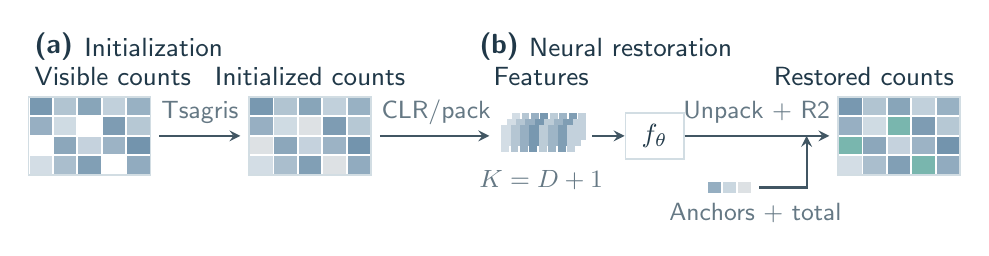
\begin{tikzpicture}[y=.8cm]
  \node[panelletter] at (0,2.43) {(a)};
  \node[label,anchor=west] at (.63,2.43) {Initialization};
  \node[panelletter] at (5.65,2.43) {(b)};
  \node[label,anchor=west] at (6.28,2.43) {Neural restoration};

  \begin{scope}[shift={(0,.40)}]\DataGrid{0}\end{scope}
  \node[label,anchor=west] at (0,1.96) {Visible counts};
  \begin{scope}[shift={(2.80,.40)}]\DataGrid{1}\end{scope}
  \node[label] at (3.575,1.96) {Initialized counts};
  \draw[flow] (1.66,1.02) -- (2.69,1.02);
  \node[small] at (2.175,1.39) {Tsagris};

  % Packed features: three offset token strips, not additional network layers.
  \begin{scope}[shift={(6.00,.77)}]
    \begin{scope}[shift={(.14,.18)}]\ChannelStrip{Observed}\end{scope}
    \begin{scope}[shift={(.07,.09)}]\ChannelStrip{Observed}\end{scope}
    \ChannelStrip{Observed}
  \end{scope}
  \node[label] at (6.51,1.96) {Features};
  \node[small] at (6.51,.31) {$K=D+1$};
  \draw[flow] (4.46,1.02) -- (5.85,1.02);
  \node[small] at (5.175,1.39) {CLR/pack};

  \node[operator,minimum width=.74cm] (f) at (7.95,1.02) {$f_\theta$};
  \draw[flow] (7.16,1.02) -- (f.west);
  \draw[flow] (f.east) -- (10.17,1.02);
  \node[small] at (9.245,1.39) {Unpack + R2};
  \begin{scope}[shift={(10.28,.40)}]\DataGrid{2}\end{scope}
  \node[label,anchor=east] at (11.83,1.96) {Restored counts};

  % Short restoration-only rail. No return route across the full figure.
  \fill[Observed!60] (8.63,.12) rectangle (8.79,.28);
  \fill[Observed!30] (8.82,.12) rectangle (8.98,.28);
  \fill[Muted!22] (9.01,.12) rectangle (9.17,.28);
  \draw[flow] (9.28,.20) -- (9.88,.20) -- (9.88,1.02);
  \node[small] at (9.23,-.20) {Anchors + total};
\end{tikzpicture}
\end{document}
